%%%%%%%%%%%%%%%%%%%%%%%%%%%%%%%%%%
\chapter{Revisão matemática}
\label{Chap:Review}
%%%%%%%%%%%%%%%%%%%%%%%%%%%%%%%%%%

\begin{fullwidth}
{\it
Algumas propriedades matemáticas importantes que serão utilizadas ao longo do curso são apresentadas abaixo.
}
\end{fullwidth}

%%%%%%%%%%%%%%%%%%%%%%%%%%%%%%
\section{Variáveis e Equações}
%%%%%%%%%%%%%%%%%%%%%%%%%%%%%%

Qualquer aplicação mais avançada que o absolutamente básico de matemática exige que usemos variáveis e equações. Uma variável é uma letra que representa um valor numérico desconhecido, ou um ``lugar'' onde devemos colocar um valor numérico qualquer. Denotamos as variáveis usando um tipo particular de fonte itálica no texto:
\begin{displaymath}
    a, b, c, d, e, f, \dots, x, y, z.
\end{displaymath}

Uma equação é uma relação de igualdade entre duas expressões matemáticas que envolvem números, operações, variáveis, etc.:
\begin{equation}
    a - b \cdot c + \dots = \frac{x}{y} + 10.
\end{equation}
%
É muito comum que equações precisem ser manipuladas de forma a isolar variáveis, porém devemos ter sempre atenção para não cometermos erros que façam com que a equação deixe de ser verdadeira. Um exemplo comum é isolar a variável $a$ na equação abaixo,
\begin{equation}
    a \cdot b = c + d,
\end{equation}
%
onde o correto é
\begin{equation}
    a = \frac{c}{b} + \frac{d}{b},
\end{equation}
%
porém um erro comum é escrever o resultado como
\begin{equation}
    a = \frac{c}{b} + d.
\end{equation}

Esse erro vem da ideia de que devemos ``passar o $b$ para o outro lado'', quando na verdade devemos nos preocupar em \emph{realizar a mesma operação de ambos os lados da equação}. Assim, para obtermos o resultado correto devemos \emph{dividir a equação original por $b$ de ambos os lados}:
\begin{align}
    a \cdot b &= c + d \\
    \frac{a\cdot b}{b} &= \frac{c + d}{b} \\
    a\cdot \frac{b}{b} &= \frac{c}{b} + \frac{d}{b} \\
    a \cdot 1 &= \frac{c}{b} + \frac{d}{b} \\
    a &= \frac{c}{b} + \frac{d}{b}.
\end{align}
%
Tenha sempre cuidado para realizar as operação adequadamente, mantendo a igualdade. Note ainda que não podemos dividir por zero, isso pode acontecer ao manipularmos equações, mas requer algum esforço no sentido de fazer errado. Abaixo ``provamos'' que 2 = 1, porém isso só é possível pois multiplicamos ambos os lados da equação por $(a-b)$, que é igual a zero devido à primeira equação:
\begin{align}
    a &= b \\
    a^2 &= ab \\
    a^2 - b^2 &= ab - b^2 \\
    (a+b)\cdot(a-b) = b\cdot(a-b) \\
    a+b = b \\
    2b = b \\
    2 = 1.
\end{align}

Um último ponto que é necessário destacar é o de que multiplicações são muito comuns em expressões, por isso geralmente omitimos o sinal de multiplicação e simplesmente grafamos as variáveis justapostas:
\begin{equation}
    a\cdot b = ab.
\end{equation}

%%%%%%%%%%%%%%%%%%%%%%%%%%%%%%%%%
\subsection{Sistemas de equações}
%%%%%%%%%%%%%%%%%%%%%%%%%%%%%%%%%

Quando trabalhamos com uma equação, podemos determinar o valor de \emph{uma} variável se a isolarmos. Em muitos tipos de áreas de aplicação podemos escrever mais que uma equação relacionando variáveis diferentes. Quando temos mais do que uma equação, podemos escrever um \emph{sistema de equações}, o que nos permite determinar o valor de mais que uma variável simultaneamente. Nem sempre um sistema de equações pode ser resolvido, porém aqueles com que vamos trabalhar nessa disciplina sempre serão \emph{sistemas possíveis determinados}.

Geralmente grafamos os sistemas como
\begin{equation}\label{Eq:ExemploSistema}
\begin{system} % x = 3, y = 5, z = 7
    3x + 4y + z &=  36\\
    4x + 8y - 3z &= 31 \\
    x + 2y -7z &= - 36.
\end{system}
\end{equation}
%
A solução desse sistema é
\begin{align*}
    x &= 3 & y &= 5 & z &= 7,
\end{align*}
%
porém, como podemos determiná-la? Temos várias possibilidades, cada uma mais adequada para um sistema específico, mas elas basicamente consistem em tomar uma das equações, fazer alguma alteração, e então usar o resultado para alterar outra equação.

A estratégia mais simples consiste em isolar uma das variáveis em uma das equações e substituir nas outras equações. Se fizermos isso com a terceira equação, por exemplo, isolando $x$, obtemos
\begin{equation}\label{Eq:SistemaSolSubsEqX}
    x = -2y + 7z -36.
\end{equation}
%
Substituindo esse resultado na primeira equação do sistema, obtemos
\begin{align}
    3x + 4y + z &=  36\\
    3\cdot(-2y + 7z -36) +4y + z &= 36\\
    -6y + 21z -108 +4y +z &= 36 \\
    -2y + 22z &= 144. \label{Eq:SistemaSolSubsEqYZ}
\end{align}
%
Substituindo a expressão que encontramos para $x$ na segunda equação do sistema, obtemos
\begin{align}
    4x + 8y - 3z &= 31 \\
    4\cdot(-2y + 7z -36) +8y - 3z &= 31 \\
    -8y + 28z - 144 + 8y - 3z &= 31 \\
    0y + 25z &= 175, \label{Eq:SistemaSolSubsEqZ}
\end{align}
%
de onde obtemos $z = 7$. Para obtermos o valor de $y$, basta utilizar o valor obtido para $z$ na Equação~\eqref{Eq:SistemaSolSubsEqYZ}. Finalmente, para obter o valor de $x$, substituimos os valores obtidos para $y$ e $z$ na Equação~\eqref{Eq:SistemaSolSubsEqX}. Note que é incomum que uma das variáveis fique com coeficiente nulo no final do processo de substituição da primeira variável isolada, como ocorreu com a Equação~\eqref{Eq:SistemaSolSubsEqZ}. Normalmente obtemos duas expressões que envolvem duas das variáveis e que formam um novo sistema que precisa então ser resolvido (sistemas com duas variáveis têm solução fácil com o método de substituição).

Outra possibilidade para solucionar o sistema \eqref{Eq:ExemploSistema} é multiplicar uma das equações por uma constante e somar em outra, visando eliminar uma das variáveis. Podemos, por exemplo, multiplicar a primeira equação por 3
\begin{align}
    3\cdot(3x + 4y + z &= 36) \\
    9x + 12y + 3z &= 108
\end{align}
%
e somar com a segunda ---~isto é, somar o lado esquerdo da primeira equação com o lado esquerdo da segunda e igualar à soma do lado direito da primeira equação com o lado direito da segunda equação~---, obtendo
\begin{align}
    (9x + 12y + 3z) + (4x + 8y - 3z) &= (108) + (31) \\
    13x + 20y + 0z &= 139.
\end{align}
%
Agora podemos multiplicar a primeira equação por 7
\begin{align}
    7\cdot(3x + 4y + z &=  36) \\
    21x + 28y + 7z &= 252
\end{align}
%
e somar à terceira
\begin{align}
    (21x + 28y + 7z) + (x + 2y -7z) &= (252) + (-36) \\
    22x + 30y + 0z &= 216.
\end{align}
%
Obtemos então um novo sistema, com somente duas variáveis:
\begin{equation}
\begin{system}
    13x + 20y &= 139 \\
    22x + 30y &= 216.
\end{system}
\end{equation}
%
Multiplicando a primeira equação desse sistema por 3 e a segunda por -2, obtemos
\begin{equation}\label{Eq:ExemploSistema2}
\begin{system}
    39x + 60y &= 417 \\
    -44 x - 60y &= -432,
\end{system}
\end{equation}
%
o que nos permite somar as equações e obter
\begin{align}
    (39x + 60y) + (-44 x - 60y) &= (417) +(-432) \\
    -5x +0y &= -15,
\end{align}
%
o que resulta em $x = 3$. Para obter o valor de $y$, basta substituir o valor de $x$ encontrado em qualquer das equações do sistema~\ref{Eq:ExemploSistema2}. Uma vez obtido o valor de $y$, podemos usar qualquer uma das equações do sistema~\ref{Eq:ExemploSistema} para determinar o valor de $z$.

Apesar de essa técnica não ter sido a mais simples que a de substituição para a solução desse exemplo, vamos ter muitos sistemas no Capítulo~\ref{Chap:Dinamica} com variáveis com coeficientes unitários, isto é, com formas similares a
\begin{equation}
\begin{system}
    F - F_{1,2} &= m_1 a \\
    F_{1,2} - F_{2,3} &= m_2 a \\
    -F_{2,3} &= m_3 a,
\end{system}
\end{equation}
%
onde a soma imediata das três equações faz com que os termos $F_{1,2}$ e $-F_{1,2}$, e $F_{2,3}$ e $-F_{2,3}$ se cancelem, resultando em
\begin{align}
    F - F_{1,2} + F_{1,2} - F_{2,3} - F_{2,3} &= m_1a + m_2a + m_3a \\
    F &= (m_1 + m_2 + m_3) a.
\end{align}
%
Note que em algumas circustâncias até mesmo dividir uma equação por outra pode ser a melhor estratégia para encontrar a solução do sistema.

%%%%%%%%%%%%%%%%%
\section{Funções}
%%%%%%%%%%%%%%%%%

\emph{O que é uma função?} Uma função é um ``objeto'' matemático que relaciona dois conjuntos de números, ou mais concretamente, dois valores numéricos que são medidos de alguma maneira. Podemos dizer, de uma maneira mais simples, que uma função é um conjunto de regras que são aplicadas a um número o transformando em outro número (ou conjunto de números). O conceito de função é fundamental para a descrição de teorias físicas pois estamos justamente interessados em descrever a relação entre grandezas.

Os conjuntos relacionados por uma função são chamados de \emph{domínio} e \emph{contradomínio}, então a função relaciona cada elemento do domínio a \emph{somente um elemento} do contradomínio. Na Figura~\ref{Fig:Funcao} mostramos o domínio à esquerda, o contradomínio à direita, e uma função $f$ que relaciona os elementos do primeiro grupo a elementos do segundo grupo. Além disso, usamos uma convenção muito comum: chamamos os elementos do domínio genericamente de $x$ e os do contradomínio de $y$ (note que não estamos nos referindo a um elemento específico quando falamos em $x$ ou em $y$, mas a qualquer um dos elementos dos respectivos grupos).
\begin{figure}[t]
\centering
\begin{tikzpicture}
\draw (0,0.5) node[above] {$x$};
\draw (3.1,0.5) node[above] {$y$};
\draw (0,-1) ellipse [x radius=12pt, y radius=40pt];
\draw (3.1,-1) ellipse [x radius=12pt, y radius=40pt];
\node [circle,draw,fill,scale=0.3] (A){};
\node [circle,draw,fill,scale=0.3] (B) [right=3cm of A] {};
\node [circle,draw,fill,scale=0.3] (C) [below=of A] {};
\node [circle,draw,fill,scale=0.3] (D) [right=3cm of C] {};
\node [circle,draw,fill,scale=0.3] (E) [below=of C] {};
\node [circle,draw,fill,scale=0.3] (F) [right=3cm of E] {};
\draw [thick, arrows={ - Stealth}]
(A) edge [bend left=45] node[above]{$f$}(B)
(C) edge [bend left=45] (D)
(E) edge [bend left=45] (F);
\end{tikzpicture}
\caption{Domínio, contradomínio e uma função $f$ que relaciona ambos.\label{Fig:Funcao}}
\end{figure}

É importante destacar que dois elementos diferentes do domínio podem apontar para um mesmo elemento do contradomínio, mas um elemento do domínio não pode apontar para dois elementos do contadomínio. Veja a Figura~\ref{Fig:DominioEContradominioFuncaoOuNao}.

\begin{marginfigure}[-3cm]
\centering
\begin{tikzpicture}[scale=1]
\draw (0,0.5) node[above] {$x$};
\draw (3.1,0.5) node[above] {$y$};
\draw (0,-1) ellipse [x radius=12pt, y radius=40pt];
\draw (3.1,-1) ellipse [x radius=12pt, y radius=40pt];
\node [circle,draw,fill,scale=0.3] (A){};
\node [circle,draw,fill,scale=0.3] (B) [right=3cm of A] {};
\node [circle,draw,fill,scale=0.3] (C) [below=of A] {};
\node [circle,draw,fill,scale=0.3] (D) [right=3cm of C] {};
\node [circle,draw,fill,scale=0.3] (E) [below=of C] {};
\node [circle,draw,fill,scale=0.3] (F) [right=3cm of E] {};
\draw [thick, arrows={ - Stealth}]
(A) edge [bend left=45] node[above]{$f$}(B)
(C) edge [bend left=45] (D)
(E) edge [bend left=45] (F);

\begin{scope}[shift={(0,-4)}]
	\draw (0,0.5) node[above] {$x$};
	\draw (3.1,0.5) node[above] {$y$};
	\draw (0,-1) ellipse [x radius=12pt, y radius=40pt];
	\draw (3.1,-1) ellipse [x radius=12pt, y radius=40pt];
	\node [circle,draw,fill,scale=0.3] (A){};
	\node [circle,draw,fill,scale=0.3] (B) [right=3cm of A] {};
	\node [circle,draw,fill,scale=0.3] (C) [below=of A] {};
	\node [circle,draw,fill,scale=0.3] (D) [right=3cm of C] {};
	\node [circle,draw,fill,scale=0.3] (E) [below=of C] {};
	\node [circle,draw,fill,scale=0.3] (F) [right=3cm of E] {};
	\draw [thick, arrows={ - Stealth}]
	(A) edge [bend left=45] node[above]{$f$}(B)
	(E) edge [bend left=45] (F);
	\draw [thick, dashed, arrows={ - Stealth}]	(C) edge [bend left=45] (B);
\end{scope}

\begin{scope}[shift={(0,-8)}]
	\draw (0,0.5) node[above] {$x$};
	\draw (3.1,0.5) node[above] {$y$};
	\draw (0,-1) ellipse [x radius=12pt, y radius=40pt];
	\draw (3.1,-1) ellipse [x radius=12pt, y radius=40pt];
	\node [circle,draw,fill,scale=0.3] (A){};
	\node [circle,draw,fill,scale=0.3] (B) [right=3cm of A] {};
	\node [circle,draw,fill,scale=0.3] (C) [below=of A] {};
	\node [circle,draw,fill,scale=0.3] (D) [right=3cm of C] {};
	\node [circle,draw,fill,scale=0.3] (E) [below=of C] {};
	\node [circle,draw,fill,scale=0.3] (F) [right=3cm of E] {};
	\draw [thick, arrows={ - Stealth}]
	(A) edge [bend left=45] node[above]{$f$}(B)
	(E) edge [bend left=45] (F);
	\draw [thick, dotted, fill, arrows={ - Stealth}, scale=0.3]	(A) edge [bend left=45] (D);
\end{scope}

\end{tikzpicture}
\caption{Embora as duas primeiras figuras representem conceitualmente uma função, a terceira não representa, pois um elemento do domínio leva a dois elementos do contradomínio.\label{Fig:DominioEContradominioFuncaoOuNao}}
\end{marginfigure}

Note que os elementos do domínio e do contradomínio podem pertencer ao conjunto dos naturais, dos racionais, dos reais, ou mesmo dos complexos. Em Física, a grande maioria dos casos são de funções com domínio e contradomínio pertencentes aos reais. Matematicamente, a função acima pode ser denotada como
\begin{equation}
    f: x \mapsto y,
\end{equation}
%
ou, o que é mais comum,
\begin{equation}
    y = f(x).
\end{equation}

%%%%%%%%%%%%%%%%%%%%%
\subsection{Gráficos}
%%%%%%%%%%%%%%%%%%%%%

\begin{marginfigure}[-1cm]
\centering
\begin{tikzpicture}
\draw (0,0.5) node[above] {$x$};
\draw (3.1,0.5) node[above] {$y$};
\draw (0,-1.3) ellipse [x radius=18pt, y radius=50pt];
\draw (3.3,-1.3) ellipse [x radius=18pt, y radius=50pt];
\node [circle,draw,scale=0.6] (A){1};
\node [circle,draw,scale=0.6] (B) [right=3cm of A] {1};
\node [circle,draw,scale=0.6] (C) [below=of A] {2};
\node [circle,draw,scale=0.6] (D) [right=3cm of C] {4};
\node [circle,draw,scale=0.6] (E) [below=of C] {3};
\node [circle,draw,scale=0.6] (F) [right=3cm of E] {9};
\draw [thick, arrows={ - Stealth}]
(A) edge [bend left=45] node[above]{$f$}(B)
(C) edge [bend left=45] (D)
(E) edge [bend left=45] (F);
\end{tikzpicture}
\caption{Utilizar um diagrama desse tipo é fácil perceber que precisamos de uma maneira mais conveniente para representar as funções.}
\end{marginfigure}

Fazer um ``desenho'' como o da Figura~\ref{Fig:Funcao} não é muito útil para reconhecermos uma função em específico, apesar de ilustrar bem o que uma função faz, ainda que genericamente. Se tivéssemos um número muito limitado de elementos, até poderia ser uma alternativa, mas uma tabela seria uma alternativa melhor. Além disso, o fato é que temos \emph{infinitos} números para relacionar. Uma técnica muito mais útil e ilustrativa\footnote[][0.5cm]{Literalmente!} é elaborar um \emph{gráfico}: usamos a distância\footnote{Essas distâncias geralmente são marcadas nos eixos do gráfico formando uma legenda do eixo em questão. Aqui vamos omitir essas marcações pois estamos mais preocupapos com a forma conceitual dos gráficos.} ao longo de dois eixos perpendiculares como representação dos valores numéricos do domínio (no eixo horizontal) e do contradomínio (no eixo vertical). Usamos essas distâncias para marcar pontos na área retangular determinada pelos eixos e obtemos pelo conjunto (infinito) de pontos uma \emph{curva}. Essa curva será diferente para cada função e podemos a usar como uma ``impressão digital'' que nos permite identificar rapidamente a função (ou pelo menos as suas principais propriedades).

\begin{figure}[h] \forceversofloat
\centering
\begin{tikzpicture}[>=Stealth,
                    scale = 1.35,
                    extended line/.style={shorten >=-#1,shorten <=-#1},
                    extended line/.default=3mm]
                   ]
 
    \draw[->, thick] (0,0) -- node[below]{Domínio} (4.3,0);
    \draw[->, thick] (0,0) -- node[above, sloped]{Contradomínio} (0,3);
    
    % Desenhar função:
    \draw[smooth,name path=plota,samples=1000,domain=0.75:3.35]
    plot(\x,{(0.75 * \x-1.5)^3 + 1.5});
    
    \draw[draw = black, fill = white] (1.5,1.447265625) circle (1mm) node[above right]{$P$};
    \fill (1.5,1.447265625) circle (0.25mm);
    
    \draw[dashed] (1.5, 1.347265625) -- (1.5,0);
    \draw[dashed] (0, 1.447265625) -- (1.4, 1.447265625);

    \draw[<->] (0.4,0) -- node[fill=white, sloped]{$v_C$} (0.4, 1.447265625);
    \draw[<->] (0, 0.25) -- node[fill=white]{$v_D$} (1.5, 0.25);
    
\end{tikzpicture}
\caption{Construção de um gráfico através de dois eixos perpendiculares: dado um elemento $x$ pertencente ao domínio, cujo valor é representado visualmente através da distância $v_D$, e um elemento $y$ correspondente do contradomínio ---~determinado através de uma função $f$~---, cujo valor é representado visualmente através da distância $v_C$, marcamos um ponto $P$. Como temos \emph{infinitos} elementos no conjunto do domínio, temos \emph{infinitos} elementos correspondentes no contradomínio. Consequentemente, temos infinitos pontos, que formam a curva contínua mostrada.\label{Fig:ConstrucaoGrafico}}
\end{figure}

\pagebreak
Na Figura~\ref{Fig:ConstrucaoGrafico} mostramos um gráfico da função 
\begin{equation}
	y = f(x) = (\np{0,75} \cdot x - \np{1,5})^3 + \np{1,5}
\end{equation}
%
para o intervalo $x \in [0.75; 3.35]$ do domínio. Nessa figura também mostramos para o mesmo intervalo de domínio as funções
\begin{align}
    y = g(x) &= \np{0.5} \\
    y = h(x) &= \np{0.4} \cdot x + 0.5 \\
    y = m(x) &= \np{0.3}\cdot\cos(1000 \cdot x) + 1,
\end{align}
%
sendo que para $m(x)$ consideramos o valor numérico de $x$ como representando um ângulo em graus.

\begin{marginfigure}[1cm]
\centering
\begin{tikzpicture}[>=Stealth,
                    scale = 1,
                    extended line/.style={shorten >=-#1,shorten <=-#1},
                    extended line/.default=3mm]
                   ]
 
    \draw[->, thick] (0,0) -- (4.3,0) node[below left]{$x$};
    \draw[->, thick] (0,0) -- (0,3) node[below left]{$y$};
    
    % Desenhar funções:
    \draw[smooth, samples=1000, domain=0.75:3.35]
    plot(\x,{(0.75 * \x-1.5)^3 + 1.5}) node[above right]{$f(x)$};
 
    \draw[smooth, dashed, samples=1000, domain=0.75:3.35]
    plot(\x,{0.5}) node[right]{$g(x)$};
    
     \draw[smooth, dashdotted, samples=1000, domain=0.75:3.35]
    plot(\x,{0.4 * \x + 0.5}) node[right]{$h(x)$};
    
     \draw[smooth, densely dotted, samples=1000, domain=0.75:3.35]
    plot(\x,{0.3 * cos(1000*\x) + 1}) node[above right]{$m(x)$};
     
\end{tikzpicture}
\caption{Gráficos que exemplificam possíveis formas para os gráficos da função posição .\label{Fig:ExemplosGraficos}}
\end{marginfigure}

Note que a função $g(x)$ é o que chamamos de uma \emph{função constante}, pois todos os elementos do domínio apontam para o mesmo elemento do contradomínio. A função $h(x)$ é uma \emph{equação da reta}, uma função muito comum em diversas áreas, incluindo a Física. Já a função $m(x)$ envolve a função cosseno, que é uma das funções trigonométricas. É importante destacar que as funções não são necessariamente escritas como \emph{polinômios}, isto é, elas não necessariamente precisam ser escritas como somas de termos com a forma $\alpha \cdot x^n$, porém isso é muito frequente e geralmente muito conveniente. A função $\cos x$, por exemplo, pode ser escrita como\footnote{Nessa série o valor numérico de $x$ representa um valor de ângulo em radianos.}
\begin{equation}
    \cos x = 1 - \frac{x^2}{2!} + \frac{x^4}{4!} - \frac{x^6}{6!} + \dots,
\end{equation}
%
onde $n!$ representa o fatorial, ou seja, $n! = n\times(n-1) \times (n-2) \times \dots \times 3 \times 2 \times 1$. Esse tipo de série é o que uma calculadora usa para determinar os valores das funções trigonométricas, porém truncando-a a um número finito de termos.

%%%%%%%%%%%%%%%%%%%%%%%%%%%%%%
\subsection{Funções em Física}
%%%%%%%%%%%%%%%%%%%%%%%%%%%%%%

Talvez você esteja se perguntando ``pra que vamos usar funções?''. Bem, pra tudo, na verdade. O conceito de função foi desenvolvido no contexto de Cálculo, são os objetos matemáticos nos quais as derivadas e integrais atuam. São as funções que são soluções do que chamamos de \emph{equações diferenciais} e as leis fundamentais da Física são sempre equações desse tipo. Assim, é fundamental que esse conceito seja dominado para que possamos estudar Física. Mesmo as relações mais simples entre variáveis físicas são descritas como funções, como a posição como função do tempo, por exemplo.

%%%%%%%%%%%%%%%%%%%%%%%%%
\section{Geometria plana}
%%%%%%%%%%%%%%%%%%%%%%%%%

Quando passarmos a trabalhar com vetores, será muito comum termos que lidar com informações envolvendo direções do espaço e os ângulos entre elas. Assim, é importante que tenhamos algumas propriedades em mente, ilustradas nas Figuras~\ref{Fig:PropAngulosRetas1} a~\ref{Fig:AlternosInternos}.
\begin{figure}
\centering
\begin{tikzpicture}

\path [draw, name path = horiz] (0,0) coordinate (start-horiz) -- (4,0) coordinate (end-horiz);
\path [draw, name path = trans] (1,-1) coordinate (start-trans) -- (3,1) coordinate (end-trans);

\path [name intersections={of = horiz and trans}] (intersection-1) coordinate (intersec);

\pic [draw, "$\alpha$", angle eccentricity=1.5] {angle = end-horiz--intersec--end-trans};
\pic [draw, "$\alpha$", angle eccentricity=1.5] {angle = start-horiz--intersec--start-trans};
\pic [draw, "$\beta$", angle eccentricity=1.5, angle radius = 3mm] {angle = start-trans--intersec--end-horiz};
\pic [draw, "$\beta$", angle eccentricity=1.5, angle radius = 3mm] {angle = end-trans--intersec--start-horiz};

\draw[fill] (start-horiz) node[left]{$A$} circle (0.5pt);
\draw[fill] (end-horiz) node[right]{$B$} circle (0.5pt);
\end{tikzpicture}
\caption{Os ângulos opostos pelo vértice (encontro das duas retas) são iguais. \label{Fig:PropAngulosRetas1}}
\end{figure}

\begin{figure}\forcerectofloat
\centering
\begin{tikzpicture}
\path[name path = sup, draw] (0,0) coordinate (start-sup) -- (4,0) coordinate (end-sup);
\path[name path = inf, draw] (0,-1.5) coordinate (start-inf) -- (4,-1.5) coordinate (end-inf);
\path[name path = trans, draw] (1, -2) coordinate (start-trans) -- (3, 0.5) coordinate (end-trans);

\draw[fill] (start-sup) node[left]{$A$} circle (0.5pt);
\draw[fill] (start-inf) node[left]{$C$} circle (0.5pt);
\draw[fill] (end-sup) node[right]{$B$} circle (0.5pt);
\draw[fill] (end-inf) node[right]{$D$} circle (0.5pt);

\path[name intersections={of= sup and trans}] (intersection-1) coordinate (int-sup);
\path[name intersections={of= inf and trans}] (intersection-1) coordinate (int-inf);

\pic[draw, "$\theta$", angle eccentricity=1.5]{angle = end-sup--int-sup--end-trans};
\pic[draw, "$\theta$", angle eccentricity=1.5]{angle = end-inf--int-inf--int-sup};

\end{tikzpicture}
\caption{Se as retas $\overline{AB}$ e $\overline{CD}$ são paralelas e uma reta transversal as atravessa, então os ângulos indicados na figura são necessariamente iguais.}
\end{figure}

\begin{figure}\forcerectofloat
\centering
\begin{tikzpicture}
\path[name path = sup, draw] (0,0) coordinate (start-sup) -- (4,0) coordinate (end-sup);
\path[name path = inf, draw] (0,-1.5) coordinate (start-inf) -- (4,-1.5) coordinate (end-inf);
\path[name path = trans, draw] (1, -2) coordinate (start-trans) -- (3, 0.5) coordinate (end-trans);

\draw[fill] (start-sup) node[left]{$A$} circle (0.5pt);
\draw[fill] (start-inf) node[left]{$C$} circle (0.5pt);
\draw[fill] (end-sup) node[right]{$B$} circle (0.5pt);
\draw[fill] (end-inf) node[right]{$D$} circle (0.5pt);

\path[name intersections={of= sup and trans}] (intersection-1) coordinate (int-sup);
\path[name intersections={of= inf and trans}] (intersection-1) coordinate (int-inf);

\pic[draw, "$\theta$", angle eccentricity=1.5]{angle = start-sup--int-sup--int-inf};
\pic[draw, "$\theta$", angle eccentricity=1.5]{angle = end-inf--int-inf--int-sup};

\end{tikzpicture}
\caption{Juntando os resultados anteriores, temos que os ângulos mostrados são iguais.\label{Fig:AlternosInternos}}
\end{figure}

%%%%%%%%%%%%%%%%%%%%%%%%%%%%%%%%%%%%%%%%%%%%%%%%%
\section{Trigonometria e funções trigonométricas}
%%%%%%%%%%%%%%%%%%%%%%%%%%%%%%%%%%%%%%%%%%%%%%%%%

No contexto de vetores, também usaremos as propriedades dos triângulos, principalmente as funções trigonométricas seno, cosseno e tangente. Por isso, relembraremos aqui as propriedades e definições mais importantes.

%%%%%%%%%%%%%%%%%%%%%%%%%%%%%%%%%%%%%%%%%%%%%%%%%%%%%%
\paragraph{Soma dos ângulos internos de um triângulo:}
%%%%%%%%%%%%%%%%%%%%%%%%%%%%%%%%%%%%%%%%%%%%%%%%%%%%%%

Note que na Figura~\ref{Fig:SomaAngulosTriangulo} a soma dos ângulos na reta superior é
\begin{equation}
    \alpha + \gamma + \beta = \degree{180}.
\end{equation}
%
Notamos também que, usando a Figura~\ref{Fig:AlternosInternos}, os ângulos internos inferiores do triângulo são iguais aos superiores externos. Logo, concluímos que a soma dos ângulos internos do triângulo também é \np[\tcdegree]{180}.

\begin{marginfigure}[-3cm]
\centering
\begin{tikzpicture}[scale = 1.2]
\draw[dashed] (0,0) coordinate (sup-starts) -- (3.5,0) coordinate (sup-ends);
\draw[dashed] (0,-1.5) coordinate (inf-starts) -- (3.5,-1.5) coordinate (inf-ends);
\draw (1,0) coordinate (A) -- (0.5,-1.5) coordinate (B) -- (3,-1.5) coordinate (C) -- cycle;

\pic[draw, "$\alpha$", angle eccentricity = 1.5] {angle = sup-starts--A--B};
\pic[draw, "$\alpha$", angle eccentricity = 1.5] {angle = C--B--A};

\pic[draw, "$\beta$", angle eccentricity = 1.5] {angle = C--A--sup-ends};
\pic[draw, "$\beta$", angle eccentricity = 1.5] {angle = A--C--B};

\pic[draw, "$\gamma$", angle eccentricity = 1.5, angle radius = 4mm] {angle = B--A--C};

\end{tikzpicture}
\caption{Soma dos ângulos de um triângulo.\label{Fig:SomaAngulosTriangulo}}
\end{marginfigure}

%%%%%%%%%%%%%%%%%%%%%%%%%%%%%%%%%
\paragraph{Teorema de Pitágoras:}
%%%%%%%%%%%%%%%%%%%%%%%%%%%%%%%%%

Ao calcularmos a área do quadrado externo na Figura~\ref{Fig:TeoremaDePitagoras}, temos
\begin{align}
    A &= (a+b)^2 \\
    &= a^2 + b^2 + 2ab.
\end{align}
%
Também podemos determinar essa área através da soma da área do quadrado interno com a área dos quatro triângulos restantes:

\begin{align}
    A &= c^2 + 4 \frac{ab}{2} \\
    &= c^2 + 2ab.
\end{align}
\begin{marginfigure}[-4cm]
\centering
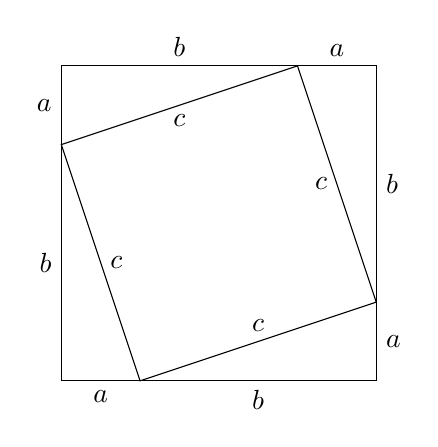
\begin{tikzpicture}
    \draw (0,0) rectangle (4,4);
    \draw (1,0) -- node[above]{$c$} (4,1) -- node[left]{$c$} (3,4) -- node[below]{$c$} (0,3) --node[right]{$c$} cycle;
    \node[below] (ad) at (0.5,0) {$a$};
    \node[right] (ar) at (4,0.5) {$a$};
    \node[above] (au) at (3.5, 4) {$a$};
    \node[left] (al) at (0, 3.5) {$a$};
    \node[below] (ad) at (2.5,0) {$b$};
    \node[right] (ar) at (4,2.5) {$b$};
    \node[above] (au) at (1.5, 4) {$b$};
    \node[left] (al) at (0, 1.5) {$b$};
\end{tikzpicture}
\caption{Através do cálculo da área chegamos no Teorema de Pitágoras. \label{Fig:TeoremaDePitagoras}}
\end{marginfigure}

\noindent{}Igualando as duas expressões para a área, temos
\begin{align}
    A &= A \\
    a^2 + b^2 + 2ab &= c^2 + 2ab \\
    a^2 + b^2 &= c^2 + 2ab - 2ab \\
    a^2 + b^2 &= c^2. \mathnote{Teorema de Pitágoras}
\end{align}


%%%%%%%%%%%%%%%%%%%%%%%%%%%%%%%%%%%%%%%%%%%%%%%%%%
\paragraph{Definição das funções trigonométricas:}
%%%%%%%%%%%%%%%%%%%%%%%%%%%%%%%%%%%%%%%%%%%%%%%%%%

No caso de um triângulo retângulo, além do Teorema de Pitágoras, também temos as relações trigonométricas seno, cosseno e tangente. Considerando o triângulo da Figura~\ref{Fig:TrianguloRetanguloDefFuncTrig}, as funções são definidas como
\begin{align}
    \sen \theta &= \frac{C_o}{h} \\
    \cos \theta &= \frac{C_a}{h} \\
    \tan \theta &= \frac{C_o}{C_a}.
\end{align}

\begin{marginfigure}[-2cm]
\centering
\begin{tikzpicture}[>=Stealth,
                    scale = 0.9,
                    interface/.style={
                                      % superfície
                                      postaction={
                                                  draw,
                                                  decorate,
                                                  decoration={
                                                              border,
                                                              angle=-45,
                                                              amplitude=0.2cm,
                                                              segment length=2mm
                                                              }
                                                 }
                                     },
    ]
     
    \draw (0,0) coordinate (O) -- node[below]{$C_a$} (4,0) coordinate (A) -- node[right]{$C_o$} (4,3) coordinate (B) -- node[sloped, above]{$h$} cycle;       

    \pic [draw, "$\theta$", angle eccentricity=1.5] {angle = A--O--B};
    
    \pic [draw, "$\cdot$", angle eccentricity=0.5, angle radius = 3mm] {angle = B--A--O};
        
\end{tikzpicture}
\caption{Triângulo retângulo. \label{Fig:TrianguloRetanguloDefFuncTrig}}
\end{marginfigure}

\noindent{}Note que as funções trigonométricas são grafadas de uma maneira um pouco diferente de outras funções genéricas, como quando escrevemos $f(x)$, $g(x)$, etc., e que omitimos os parentesis. A omissão dos parentesis não é obrigatória, no entanto, muitas vezes escrevemos $\sen(\theta)$, $\cos(\theta)$, ou $\tan(\theta)$. Já o uso de uma fonte ``normal'' ao invés de itálica é algo comum ao escrevermos diversas funções ``não-genéricas'', como o logarítimo $\log(x)$, ou o logarítimo natural $\ln(x)$, por exemplo. Nas Figuras~\ref{Fig:GraphSenCos} e~\ref{Fig:GraphTan} mostramos os gráficos das funções trigonométricas.

\begin{figure}
\centering
\begin{tikzpicture}[>=Stealth]
    \draw[->] (0,0) -- (10,0) node[below left]{$\theta$};
    
    \draw[->] (0, -1.5) -- (0,1.5);
    
    % Desenhar funções seno e cosseno:
    \draw[dashed, smooth, samples=1000, domain=0:8.5]
    plot(\x,{sin(100*\x)}) node[right]{$\sen(\theta)$};
    
    \draw[dashdotted, smooth, samples=1000, domain=0:8.5]
    plot(\x,{cos(100*\x)}) node[right]{$\cos(\theta)$};
    
    \draw[densely dotted] (0,1) node[left]{1} -- (8.5,1);
    \draw[densely dotted] (0,-1) node[left]{-1} -- (8.5,-1);
    
    \foreach \i in {0,0.9,...,9.5} \draw[draw = black, fill = white] (\i, 0) circle (1pt);
    
\end{tikzpicture}
\caption{Gráfico das funções trigonométricas seno e cosseno. Os pequenos círculos no eixo horizontal marcam os ângulos de \degree{0}, \degree{90}, \degree{180}, etc. Note que ambas as funções são limitadas ao intervalo $[-1; 1]$ no conjunto do contradomínio, isto é, no eixo vertical.\label{Fig:GraphSenCos}}
\end{figure}

\begin{figure}\forcerectofloat
\centering
\begin{tikzpicture}[>=Stealth,yscale=0.7]
    \draw[->] (0,0) -- (10,0) node[below left]{$\theta$};
    
    \draw[->] (0, -3.5) -- node[above, sloped, very near end]{$\tan\theta$} (0,3.5);
        
    \draw[dashed, smooth, samples=1000, domain=0:0.7]
    plot(\x,{tan(100*\x)});
    \draw[smooth, samples=1000, domain=0:0.6]
    plot(\x,{tan(100*\x)});
    
    \draw[dashed, smooth, samples=1000, domain=1.1:2.5]
    plot(\x,{tan(100*\x)});
    \draw[smooth, samples=1000, domain=1.2:2.4]
    plot(\x,{tan(100*\x)});
    
    \draw[dashed, smooth, samples=1000, domain=2.9:4.3]
    plot(\x,{tan(100*\x)});
    \draw[smooth, samples=1000, domain=3.0:4.2]
    plot(\x,{tan(100*\x)});
    
    \draw[dashed, smooth, samples=1000, domain=4.7:6.10]
    plot(\x,{tan(100*\x)});
    \draw[smooth, samples=1000, domain=4.8:6.0]
    plot(\x,{tan(100*\x)});
    
    \draw[dashed, smooth, samples=1000, domain=6.5:7.9]
    plot(\x,{tan(100*\x)});
    \draw[smooth, samples=1000, domain=6.6:7.8]
    plot(\x,{tan(100*\x)});
    
    \draw[dashed, smooth, samples=1000, domain=8.3:9.7]
    plot(\x,{tan(100*\x)});
    \draw[smooth, samples=1000, domain=8.4:9.6]
    plot(\x,{tan(100*\x)});
    
    \foreach \i in {0,0.9,...,9.5}{
        \draw[draw = black, fill = white] (\i, 0) circle (1pt);
        \draw[densely dotted] (\i, 3.5) -- (\i, -3.5);
    }
    
\end{tikzpicture}
\caption{Gráfico das funções tangente. Os pequenos círculos no eixo horizontal marcam os ângulos de \degree{0}, \degree{90}, \degree{180}, etc. As linhas pontilhadas verticais marcam os ângulos de \degree{90} e \degree{270}, bem como seus múltiplos, onde a função tangente vai ao infinito.\label{Fig:GraphTan}}
\end{figure}

%%%%%%%%%%%%%%%%%%%%%%%%%%%%%%%%%%%%%%%%%%%%%
\paragraph{Funções trigonométricas inversas:}
%%%%%%%%%%%%%%%%%%%%%%%%%%%%%%%%%%%%%%%%%%%%%

Sabemos que uma função associa elementos do conjunto domínio a elementos do conjunto contradomínio. Muitas vezes é possível determinar uma segunda função que associa os elementos do contradomínio aos elementos do conjunto original, e denominamos tal função como \emph{função inversa} da função original. Note que nem sempre é possível determinar uma função inversa, ou podemos determiná-la com algumas restrições.

No caso das funções trigonométricas, podemos escrever funções inversas que retornam valores de ângulo no intervalo $[-\degree{90}; \degree{90}]$ para a inversa do seno, $[\degree{0}; \degree{180}]$ para a inversa do cosseno, e $[-\degree{90}; \degree{90}]$ para a inversa da tangente. Note que um ângulo é negativo quando é medido no sentido horário. As funções trigonométricas inversas costumam ser denominadas como ``arco seno'', ``arco cosseno'', e ``arco tangente'', sendo grafadas como $\arcsen(x)$, $\arccos(x)$, e $\arctan(x)$, respectivamente. Alternativamente, as funções podem ser grafadas como $\textrm{sen}^{-1}(x)$, $\textrm{cos}^{-1}(x)$, e $\textrm{tan}^{-1}(x)$, principalmente quando existe alguma restrição de espaço, como ao rotular os botões de uma calculadora. Nas Figuras~\ref{Fig:FuncTrigInvSen} a~\ref{Fig:FuncTrigInvTan} temos os gráficos das funções trigonométricas inversas.

\begin{figure}
\centering
\begin{tikzpicture}[>=Stealth]
    \draw[->] (-5,0) -- (5,0) node[above]{$x = \arcsen\theta$};
    
    \draw[->] (0, -2.25) -- (0,2.25) node[below left]{$\theta$};
        
    \draw[dashed, smooth, samples=1000, domain=-4:4]
    plot(\x,{1.5 * asin(\x/4) / 90});
    
    \draw[|-|] (-4,0) node[below]{\clap{$-1$}} -- (4,0) node[below]{\clap{$1$}};
    \draw[|-|] (0,1.5) node[left]{\degree{90}} -- (0,-1.5) node[right]{-\degree{90}};
    
    \draw[densely dotted] (-4,0) -- (-4,-1.5) -- (0, -1.5);
    \draw[densely dotted] (4,0) -- (4,1.5) -- (0,1.5);
    
    
\end{tikzpicture}
\caption{Gráfico da função $\arcsen(x)$. Note que a função toma valores de seno, compreendidos no intervalo $[-1; 1]$, e devolve valores de ângulo compreendidos entre $-\degree{90}$ e $\degree{90}$. \label{Fig:FuncTrigInvSen}}
\end{figure}

\begin{figure}\forceversofloat
\centering
\begin{tikzpicture}[>=Stealth]
    \draw[->] (-5,0) -- (5,0) node[above]{$x = \arccos\theta$};
    
    \draw[->] (0, -0.5) -- (0,4) node[below left]{$\theta$};
        
    \draw[dashed, smooth, samples=1000, domain=-4:4]
    plot(\x,{1.5 * acos(\x/4) / 90});
    
    \draw[|-|] (-4,0) node[below]{\clap{$-1$}} -- (4,0) node[below]{\clap{$1$}};
    \draw[-|] (0,0) node[below left]{\degree{0}} -- (0,3) node[below left]{\degree{180}};
    
    \draw[densely dotted] (4,0) -- (4,3) -- (-4,3) -- (-4,0);
    
    
\end{tikzpicture}
\caption{Gráfico da função $\arccos(x)$. Note que a função toma valores de cosseno, compreendidos no intervalo $[-1; 1]$, e devolve valores de ângulo compreendidos entre $\degree{0}$ e $\degree{180}$. \label{Fig:FuncTrigInvCos}}
\end{figure}

\begin{figure}\forceversofloat
\centering
\begin{tikzpicture}[>=Stealth,
                    xscale = 0.5
                   ]
    \draw[->] (-10,0) -- (10,0) node[above]{$x = \arctan\theta$};
    
    \draw[->] (0, -2.25) -- (0,2.25) node[below left]{$\theta$};
        
    \draw[dashed, smooth, samples=1000, domain=-9.5:9.5]
    plot(\x,{1.5 * atan(\x) / 90});

    \draw[smooth, samples=1000, domain=-8:8]
    plot(\x,{1.5 * atan(\x) / 90});
    
    \draw[|-|] (0,1.5) node[below left]{\degree{90}} -- (0,-1.5) node[below left]{-\degree{90}};
    
    \draw[densely dotted] (-9,-1.5) -- (9,-1.5);
    \draw[densely dotted] (-9,1.5) -- (9,1.5);
    
    \foreach \x in {2, 4, ..., 8} \draw (\x,0) -- (\x, -0.1) node[below]{$\x$};
    \foreach \x in {2, 4, ..., 8} \draw (-\x,0) -- (-\x, -0.1) node[below]{$-\x$};
    
\end{tikzpicture}
\caption{Gráfico da função $\arctan(x)$. Note que a função toma valores de tangente, compreendidos no intervalo $[-\infty; \infty]$, e devolve valores de ângulo compreendidos entre $-\degree{90}$ e $\degree{90}$.  \label{Fig:FuncTrigInvTan}}
\end{figure}

\FloatBarrier
%%%%%%%%%%%%%%%%%%%%%%%%%%%%%%%%%%%
\paragraph{Círculo trigonométrico:}
%%%%%%%%%%%%%%%%%%%%%%%%%%%%%%%%%%%

Uma ferramenta que ajuda muito a entender as propriedades das funções trigonométricas é o que chamamos de \emph{círculo trigonométrico}. Ela consiste em um círculo de raio unitário onde interpretamos geometricamente as propriedades das funções. Veja a Figura~\ref{Fig:CirculoTrigonometrico}. Como escolhemos o raio como unitário, os valores de seno e cosseno correspondem ao próprio comprimento dos respectivos catetos, uma vez que a hipotenusa é igual ao raio, que é 1. Também podemos visualizar a tangente no eixo à direita, \emph{tangente} ao círculo. O valor é igual à distância entre o ponto de interseção entre o eixo que determina o ângulo (eixo tracejado na figura) e a própria reta das tangentes.

\begin{figure}
\centering
\begin{tikzpicture}[>=Stealth,
                    scale = 0.85
                   ]

    \draw[name path = horiz] (-5,0) -- (5,0) coordinate (A);
    \draw[name path = vert] (0, -5) -- (0, 5);
    
    \draw (0,0) coordinate (O) circle (4cm);
    
    \path [name path = radius] (50:-5) -- (50:8);
    \path [name path = tan, draw] (4,-5) -- (4,5);
    
    \draw[dashed, name intersections={of=radius and tan}] (50:-5) -- (intersection-1) coordinate (tan);
    \draw[thick] (O) -- (50:4) coordinate (P);
    
    \path [name path = phoriz] (P) -- +(-4,0);
    \path [name path = pvert] (P) -- +(0,-4);
    
    \draw [dashdotted, name intersections={of=pvert and horiz}] (P) -- (intersection-1) coordinate (cos);
    \draw [dashdotted, name intersections={of=phoriz and vert}] (P) -- (intersection-1) coordinate (sen);
    
    \draw [|<->|] (0, -0.3) -- node[fill = white]{$\cos\theta$} ([yshift=-3mm]cos);
    \draw [|<->|] (-0.3, 0) -- node[sloped, fill = white]{$\sen\theta$} ([xshift=-3mm]sen);
    
    \draw[<->|] (4.3,0) -- node[sloped, rotate = 180, fill = white]{$\tan\theta$} ([xshift=3mm]tan);
    
    \pic [draw, "$\theta$", angle eccentricity = 1.5]{angle = A--O--P};
    
\end{tikzpicture}
\caption{Círculo trigonométrico.  \label{Fig:CirculoTrigonometrico}}
\end{figure}

Devemos destacar ainda que o eixo horizontal, onde verificamos os valores de cosseno, apresenta valores positivo à direita da origem\footnote{A origem é a interseção entre o eixo vertical e o horizontal.} e negativos à esquerda desse ponto. Já o eixo vertical, que determina os valores de seno, tem valores positivos acima da origem e negativos abaixo dela. O eixo das tangentes é positivo acima de sua interseção com o eixo horizontal e negativo abaixo dele. Assim, os quadrantes apresentam sinais diferentes para as funções trigonométricas.


\begin{figure*}
\centering
\begin{tikzpicture}[>=Stealth,
                    scale = 1.5
                   ]

    \draw[name path = horiz] (-1.5,0) -- (1.5,0);
    \draw[name path = vert] (0, -1.5) node[below]{$\sin\theta$} -- (0, 1.5);
    
    \draw (0,0) circle (1cm);
    
    \fill[pattern = north west lines] (0,0) -- (1,0) arc[start angle=0, end angle = 180, radius = 1cm] (-1,0) -- cycle;
    
%    \node[circle, radius = 2mm, fill = white] (Q1) at (45:0.5) {$+$};
%    \node[circle, radius = 2mm, fill = white] (Q2) at (135:0.5) {$+$};
%    \node[circle, radius = 2mm, fill = white] (Q3) at (225:0.5) {$-$};
%    \node[circle, radius = 2mm, fill = white] (Q4) at (315:0.5) {$-$};
    
    \begin{scope}[shift={(3.5,0)}]
    
        \draw[name path = horiz] (-1.5,0) -- (1.5,0);
        \draw[name path = vert] (0, -1.5) node[below]{$\cos\theta$} -- (0, 1.5);
        
        \draw (0,0) circle (1cm);
        
        \fill[pattern = north west lines] (0,0) -- (0,-1) arc[start angle=-90, end angle = 90, radius = 1cm] (0,1) -- cycle;

    \end{scope}
    
    \begin{scope}[shift={(7,0)}]
    
        \draw[name path = horiz] (-1.5,0) -- (1.5,0);
        \draw[name path = vert] (0, -1.5) node[below]{$\tan\theta$} -- (0, 1.5);
        
        \draw (0,0) circle (1cm);
        
        \fill[pattern = north west lines] (0,0) -- (1,0) arc[start angle=0, end angle = 90, radius = 1cm] (0,1) -- cycle;
        \fill[pattern = north west lines] (0,0) -- (-1,0) arc[start angle=180, end angle = 270, radius = 1cm] (0,-1) -- cycle;
    \end{scope}
    
\end{tikzpicture}
\caption{Quadrantes e sinais das fuções trigonométricas. As regiões destacadas têm valores positivos da função trigonométrica correspondente. \label{Fig:SinaisQuadrantesFuncTrig}}
\end{figure*}

%%%%%%%%%%%%%%%%%%%%%%%%%%%%%%%%%%%%%%%%%%%%%%%%
\paragraph{Relações de funções trigonométricas:}
%%%%%%%%%%%%%%%%%%%%%%%%%%%%%%%%%%%%%%%%%%%%%%%%

Existem diversas relações entre funções trigonométricas:
\begin{align}
	\sen^2\theta + \cos^2\theta &= 1 \\
	\sen (2\theta) &= 2\sen \theta \cos \theta \\
	\cos(2\theta) &= \cos^2\theta - \sen^2 \theta \\
	&= 1 - 2\sen^2\theta,
\end{align}
%
dentre inúmeras outras.

A primeira, em especial, pode ser verificada de uma maneira muito simples, basta usarmos a definição das próprias funções seno e cosseno:
\begin{align}
	\sen^2\theta + \cos^2\theta &= 1 \\
	\left(\frac{C_o}{h}\right)^2 + \left(\frac{C_a}{h}\right)^2 &= 1.
\end{align}
%
Note que ao multiplicarmos ambos os lados da equação por $h^2$ obtemos o Teorema de Pitágoras,
\begin{equation}
	C_o^2 + C_a^2 = h^2,
\end{equation}
%
o que mostra que a relação inicial é verdadeira.



%%%%%%%%%%%%%%%%%%%%%%%%%
%\section{Áreas e volumes}
%%%%%%%%%%%%%%%%%%%%%%%%%






